\documentclass[fleqn,10pt]{wlscirep}
\usepackage[utf8]{inputenc}
\usepackage[T1]{fontenc}
\title{Scientific Reports Title to see here}

\author[1,*]{Alice Author}
\author[2]{Bob Author}
\author[1,2,+]{Christine Author}
\author[2,+]{Derek Author}
\affil[1]{Affiliation, department, city, postcode, country}
\affil[2]{Affiliation, department, city, postcode, country}

\affil[*]{corresponding.author@email.example}

\affil[+]{these authors contributed equally to this work}

%\keywords{Keyword1, Keyword2, Keyword3}

\begin{abstract}
Example Abstract. Abstract must not include subheadings or citations. Example Abstract. Abstract must not include subheadings or citations. Example Abstract. Abstract must not include subheadings or citations. Example Abstract. Abstract must not include subheadings or citations. Example Abstract. Abstract must not include subheadings or citations. Example Abstract. Abstract must not include subheadings or citations. Example Abstract. Abstract must not include subheadings or citations. Example Abstract. Abstract must not include subheadings or citations.
\end{abstract}
\begin{document}

\flushbottom
\maketitle
% * <john.hammersley@gmail.com> 2015-02-09T12:07:31.197Z:
%
%  Click the title above to edit the author information and abstract
%
\thispagestyle{empty}

\noindent Please note: Abbreviations should be introduced at the first mention in the main text – no abbreviations lists. Suggested structure of main text (not enforced) is provided below.

\section*{Introduction}

The Introduction section, of referenced text\cite{Figueredo:2009dg} expands on the background of the work (some overlap with the Abstract is acceptable). The introduction should not include subheadings.

\section*{Results}

Up to three levels of \textbf{subheading} are permitted. Subheadings should not be numbered.

\subsection*{Subsection}

Example text under a subsection. Bulleted lists may be used where appropriate, e.g.

\begin{itemize}
\item First item
\item Second item
\end{itemize}

\subsubsection*{Third-level section}
 
Topical subheadings are allowed.

\section*{Discussion}

The Discussion should be succinct and must not contain subheadings.

\section*{Methods}

Topical subheadings are allowed. Authors must ensure that their Methods section includes adequate experimental and characterization data necessary for others in the field to reproduce their work.

\bibliography{sample}

\noindent LaTeX formats citations and references automatically using the bibliography records in your .bib file, which you can edit via the project menu. Use the cite command for an inline citation, e.g.  \cite{Hao:gidmaps:2014}.

For data citations of datasets uploaded to e.g. \emph{figshare}, please use the \verb|howpublished| option in the bib entry to specify the platform and the link, as in the \verb|Hao:gidmaps:2014| example in the sample bibliography file.

\section*{Acknowledgements (not compulsory)}

Acknowledgements should be brief, and should not include thanks to anonymous referees and editors, or effusive comments. Grant or contribution numbers may be acknowledged.

\section*{Author contributions statement}

Must include all authors, identified by initials, for example:
A.A. conceived the experiment(s),  A.A. and B.A. conducted the experiment(s), C.A. and D.A. analysed the results.  All authors reviewed the manuscript. 

\section*{Additional information}

To include, in this order: \textbf{Accession codes} (where applicable); \textbf{Competing interests} (mandatory statement). 

The corresponding author is responsible for submitting a \href{http://www.nature.com/srep/policies/index.html#competing}{competing interests statement} on behalf of all authors of the paper. This statement must be included in the submitted article file.

\begin{figure}[ht]
\centering
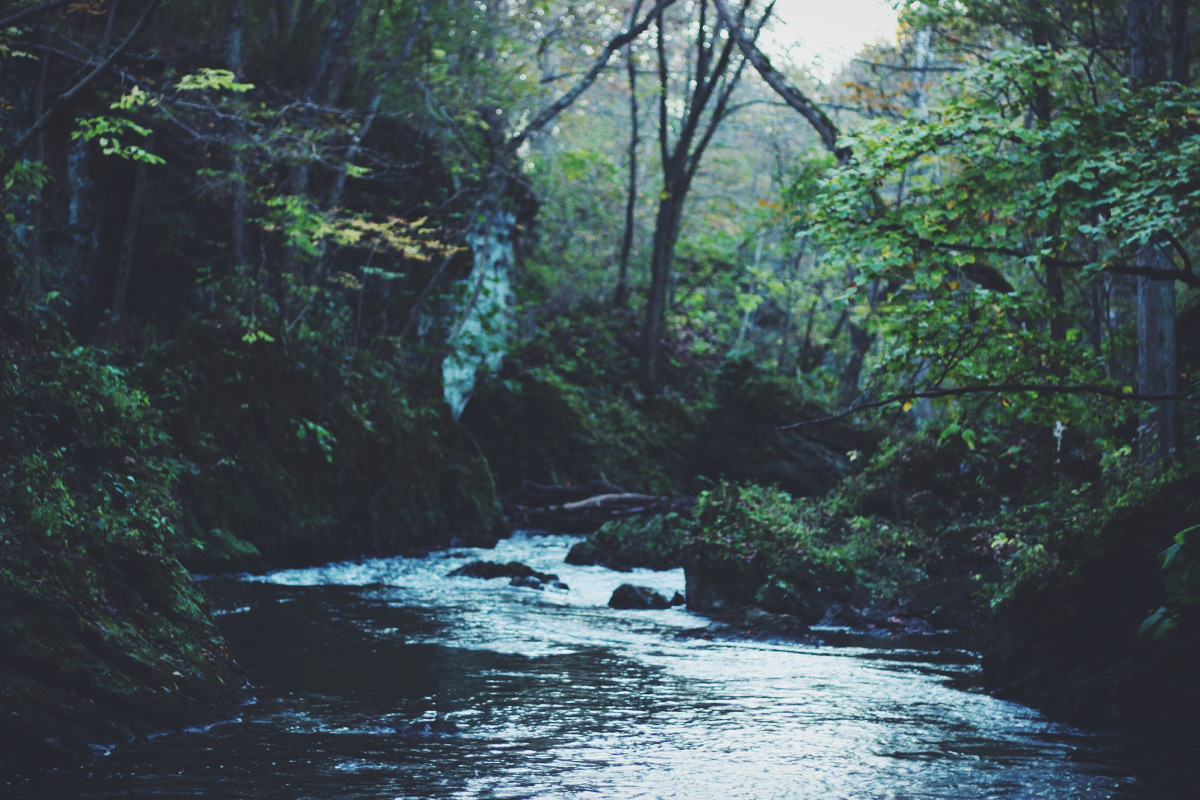
\includegraphics[width=\linewidth]{stream}
\caption{Legend (350 words max). Example legend text.}
\label{fig:stream}
\end{figure}

\begin{table}[ht]
\centering
\begin{tabular}{|l|l|l|}
\hline
Condition & n & p \\
\hline
A & 5 & 0.1 \\
\hline
B & 10 & 0.01 \\
\hline
\end{tabular}
\caption{\label{tab:example}Legend (350 words max). Example legend text.}
\end{table}

Figures and tables can be referenced in LaTeX using the ref command, e.g. Figure \ref{fig:stream} and Table \ref{tab:example}.

\end{document}